\documentclass[a4paper,11pt]{article}
\input{/home/tof/Documents/Cozy/latex-include/preambule_lua.tex}
\newcommand{\showprof}{show them}  % comment this line if you don't want to see todo environment
\fancyhead[L]{Image numérique}
\newdate{madate}{10}{09}{2020}
%\fancyhead[R]{\displaydate{madate}} %\today
\fancyhead[R]{Seconde - SNT}
%\fancyhead[R]{Première - NSI}
%\fancyhead[R]{Terminale - NSI}
\fancyfoot[L]{~\\Christophe Viroulaud}
\AtEndDocument{\label{lastpage}}
\fancyfoot[C]{\textbf{Page \thepage/\pageref{lastpage}}}
\fancyfoot[R]{\includegraphics[width=2cm,align=t]{/home/tof/Documents/Cozy/latex-include/cc.png}}
\usepackage{tikz}

\begin{document}
\begin{Form}
\section{Problématique}
Les images numériques sont composées de pixels. Pris séparément il ne représente qu'un point coloré, mais en alignant un grand nombre de points, nous pouvons construire des formes. 
\begin{center}
\shadowbox{\parbox{14cm}{\centering Comment construire une image numérique dans la mémoire d'un ordinateur?}}
\end{center}
\section{Image matricielle}
\subsection{Définition}
Il existe deux manières de construire une image numérique:
\begin{itemize}
\item les images vectorielles,
\item les images matricielles.
\end{itemize}
Nous nous concentrerons sur cette seconde méthode. Nous pouvons voir une matrice comme une grille où chaque pixel est repéré par ses coordonnées (figure \ref{matrice}).
\begin{center}
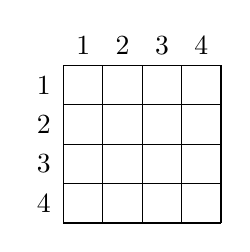
\begin{tikzpicture}[scale=0.5]
\draw (0,0) grid (4,4);

\draw (-0.5,3.5) node{1};
\draw (-0.5,2.5) node{2};
\draw (-0.5,1.5) node{3};
\draw (-0.5,0.5) node{4};
\draw (0.5,4.5) node{1};
\draw (1.5,4.5) node{2};
\draw (2.5,4.5) node{3};
\draw (3.5,4.5) node{4};
\end{tikzpicture}
\captionof{figure}{Matrice}
\label{matrice}
\end{center}
Le format \emph{bitmap (bmp)} est une image matricielle. Les formats jpg ou png également
\subsection{Construire une image}
\subsubsection{Noir et blanc}
\section{Métadonnées}
\url{https://www.verexif.com}
\url{http://exif.regex.info/exif.cgi}

\end{Form}
\end{document}